%intro needs more work
Σ' αυτό το κεφάλαιο θα παρουσιάσουμε τα πειραματικά αποτελέσματα που αφορούν την Non-Blocking point-to-point επικοινωνία για αρχιτεκτονικές NUMA και UMA. Αρχικά παραθέτουμε τις εφαρμογές και μετρικές που χρησιμοποιήσαμε για να εξετάσουμε τη συμπεριφορά των μοντέλων. Μετέπειτα αναφερόμαστε στα αποτελέσματα και στις προσπάθειες μας για να τα βελτιώσουμε.

\section{Εφαρμογές για εξαγωγή του συνόλου αξιολόγησης}
\paragraph{}
Σε αναλογία με το training set, που προορίζεται για την εκπαίδευση των μοντέλων επικοινωνίας, το σύνολο αξιολόγησης (testing set) περιέχει δείγματα που αποσκοπούν στην εξέταση της ακρίβειας των μοντέλων μας. Εξετάσαμε δύο εφαρμογές, με communication patterns αρκετά συνήθη στις παράλληλες εφαρμογές, για να έχουμε μία γενική εικόνα αναφορικά με τη συμπεριφορά των μοντέλων.
\subsection{3D-Jacobi}
\paragraph{}
Η πρώτη εφαρμογή ήταν μία παράλληλη υλοποίηση της επίλυση ενός προβλήματος διάδοσης θερμότητας σε ένα τρισδιάστατο χωρίο με χρήση της επαναληπτικής μεθόδου Jacobi. Αρχικά, οι MPI διεργασίες τοποθετούνται σε ένα εικονικό 3D καρτεσιανό πλέγμα και με βάση τη θέση τους, το αρχικό χωρίο χωρίζεται σε 3D υποχωρία και κατανέμεται σε αυτές. Κάθε MPI διεργασία έχει, ανάλογα με τη θέση της στο πλέγμα, κάποιες γειτονικές διεργασίες με τις οποίες χρειάζεται να ανταλλάξει δεδομένα.  Συγκεκριμένα, μία διεργασία καλείται να στείλει σε κάθε γειτονική της, τη 2D εδρα που συνορεύει με αυτή βλ. Σχήμα \ref{fig:halo3d}\footnote{http://www.slideshare.net/DevCentralAMD/cc-4005-joshuamora-28493997}. Αντίστοιχα, τον ίδιο όγκο δεδομένων πρέπει να λάβει από αυτές. Αυτού του τύπου μοτίβα επικοινωνίας, όπου γειτονικές διεργασίες με βάση τη κατανομή ενός χωρίου ανταλλάσσουν συμμετρικά δεδομένα, ονομάζονται Halo. Είναι εμφανές ότι το μέγεθος των μηνυμάτων εξαρτάται από τη γεωμετρία του 3D εικονικού πλέγματος και το μέγεθος του αρχικού χωρίου. Σε περίπτωση που το πλέγμα είναι ασύμμετρο, η διάσταση με τις λιγότερες διεργασίες, θα απαιτεί περισσότερη επικοινωνία καθώς οι γειτονικές 2D έδρες είναι μεγαλύτερες. Είχαμε τη δυνατότητα να ορίσουμε τις διαστάσεις του 3D πλέγματος όπως και τις διαστάσεις του αρχικού χωρίου. Πρόκειται για επαναληπτική μέθοδο, με κάθε επανάληψη να εμφανίζει το ίδιο communication pattern και την επικοινωνία που περιγράψαμε. Υπολογίζαμε την πρόβλεψη για μία επανάληψη, $\hat{t}_{iter}$, και την τελική πρόβλεψη μέσω του γινομένου $\hat{t}_{total}= iterations \times \hat{t}_{iter}$. Εκτελέσαμε την εφαρμογή για σωρεία μεγεθών χωρίου και mappings με αποτέλεσμα την εξαγωγή αρκετών σημείων και την πιο σφαιρική αξιολόγηση των μοντέλων. Λεπτομέρειες για τις παραμέτρους εκτέλεσης και τον αριθμό των εξαγόμενων σημείων δίνονται στον Πίνακα \ref{table:par_jacobi}.


\begin{figure}[ht]
    \centering
    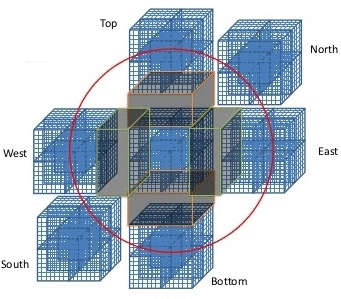
\includegraphics[width=0.55\textwidth]{./images/halo3d.png}
    \caption{Ανταλλαγή Halo-3D}
    \label{fig:halo3d}
\end{figure}
\begin{table} \footnotesize

\centering
\caption{Λεπτομέρειες Εκτέλεσης Jacobi-3D}
\label{table:par_jacobi}
\begin{tabular}{c||c|c}
\multirow{2}{*}{Παράμετρος} & \multicolumn{2}{c}{Αρχιτεκτονική}                                                     \\
                            & UMA                                       & NUMA                                      \\ \hline \hline
N                           & 1                                         & 2-4                                       \\
PPN                         & 2-8                                       & 1-8                                       \\
Domain Size                 & $50^3,100^3,200^3,300^3,400^3,...,1000^3$ & $50^3,100^3,200^3,300^3,400^3,...,1000^3$ \\ 
Iterations                  & 200                                       & 200                                       \\ \hline	
\textbf{\#samples }                  & 66                                        & 176                                      
\end{tabular}
\end{table}





\subsection{LULESH}
\paragraph{}
H δεύτερη εφαρμογή ήταν το Livermore Unstructured Lagrangian Explicit Shock Hydrodynamics (LULESH) \cite{LULESH}. Σε αντίθεση με το 3D-Jacobi, το LULESH παρουσιάζει τρεις φάσεις επικοινωνίας σε κάθε επανάληψη. Η πρώτη φάση, περιλαμβάνει την ανταλλαγή 26 μηνυμάτων, σε ένα 3D-Halo πρότυπο, για την επικοινωνία κάποιων διανυσμάτων δυνάμεων. Η ουσιώδες διαφορά με το 3D-Jacobi είναι ότι τα μηνύματα αυτά δεν είναι ίσου μεγέθους. Η δεύτερη φάση, αφορά την ανταλλαγή μηνυμάτων 6 σημείων, ξανά σε ένα 3D-Halo πρότυπο για την επικοινωνία του ιξώδες του ρευστού, ενώ η τρίτη την επικοινωνία ενός τρισδιάστατου μετώπου κύματος και πάλι 26 σημείων, με θέσεις και ταχύτητες. Προβλέπουμε κάθε μία από αυτές ξεχωριστά, και προσθέτουμε τα αποτελέσματα για να υπολογίσουμε την πρόβλεψη για μία επανάληψη, $\hat{t}_{iter}$. Για την τελική πρόβλεψη,  $\hat{t}$, πολλαπλασιάζουμε το αποτέλεσμα με τον αριθμό των επαναλήψεων. Επιπρόσθετα η MPI υλοποίηση του LULESH εκτελεί ένα \textit{Allreduce} collective για ένα αριθμό κινούμενης υποδιαστολής διπλής ακρίβειας. Με αυτό εξετάζουμε και τη συμπεριφορά των μοντέλων για την collective  επικοινωνία. Λεπτομέρειες για τις παραμέτρους εκτέλεσης δίνονται στον Πίνακα \ref{table:par_lulesh}. Δυστυχώς, η εφαρμογή απαιτεί ο αριθμός των MPI διεργασιών, να είναι αποτέλεσμα κυβικού εκθέτη, γεγονός που περιόριζε τα configurations που μπορούσαμε να εξετάσουμε. Τέλος, σημειώνουμε ότι ο μετρούμενος χρόνος εκτέλεσης, $t$, υπολογίζεται αθροιστικά για κάθε φάση ξεχωριστά, πάνω από όλες τις επαναλήψεις και για τις δύο εφαρμογές.

\begin{table} \footnotesize
\centering
\caption{Λεπτομέρειες Εκτέλεσης LULESH}
\label{table:par_lulesh}
\begin{tabular}{c||c|c}
\multirow{2}{*}{Παράμετρος} & \multicolumn{2}{c}{Αρχιτεκτονική}                                                           \\ 
                            & UMA                                          & NUMA                                         \\ \hline \hline
N                           & 1                                            & 2/4                                          \\
PPN                         & 8                                          & 4/2                                          \\
Domain Size                 & $50^3,60^3,70^3,80^3,90^3,100^3,150^3,200^3$ & $50^3,60^3,70^3,80^3,90^3,100^3,150^3,200^3$ \\
Iterations                  & 200                                          & 200                                          \\ \hline
\textbf{\#samples}                   & 8                                            & 16                                          
\end{tabular}
\end{table}
\section{Μετρικές Αξιολόγησης}
\paragraph{}
Για την αξιολόγηση των μοντέλων μας χρησιμοποιήσαμε τέσσερις μετρικές. Η πρώτη ήταν το σχετικό σφάλμα για κάθε πρόβλεψη, που υπολογίζεται ως ακολούθως:
\begin{align*}
e = \frac{\hat{t}-t}{t}
\end{align*}
Μας έδινε μία αναλυτική εικόνα για τη συμπεριφορά του μοντέλου για κάθε σημείο ξεχωριστά. Έτσι μπορούσαμε να το χρησιμοποιήσουμε για να κάνουμε παρατηρήσεις και να αποφασίσουμε τα επόμενα βήματα της δουλειάς μας.
\paragraph{}
Ωστόσο, καθώς είναι μετρική που υπολογίζεται για την κάθε πρόβλεψη ξεχωριστά χρησιμοποιήσαμε και τη μέση τιμή των απόλυτων τιμών της σαν μετρική αξιολόγησης που μας δίνει μία πιο γενική εικόνα για την ακρίβεια των προβλέψεων. Έστω, $m$ ο αριθμός των προβλέψεων και $e_i$ η τιμή του σχετικού σφάλματος για την i-ιοστή πρόβλεψη. Η μετρική υπολογίζεται ως εξής:
\begin{align*}
\mu = avg(|e_i|), 1\leq i \leq m
\end{align*}
\paragraph{}
Η τρίτη μετρική ήταν το Rank Correlation Coefficient(RCC). Παίρνει τιμές ανάμεσα στο μηδέν και το ένα και ορίζει πόσο καλά προβλέπει το μοντέλο τη διάταξη μεταξύ των μετρούμενων χρόνων. Έτσι, μπορούμε να αποφανθούμε για το κατά πόσο το μοντέλο διακρίνει διαφορές ανάμεσα στα σημεία που προέβλεψε και πόσο καλά θα λειτουργούσε σε σενάρια βελτιστοποίησης. Έστω, $t_i, 1\leq i \leq m$ ο μετρούμενος χρόνος επικοινωνίας και $\hat{t}_i$ η αντίστοιχη πρόβλεψη για m σημεία. Το RCC ορίζεται σαν:
\begin{align*}
RCC = \sum_{1\leq i \leq m} \sum_{1\leq i \leq m} concordant_{ij}/ \frac{m(m-1)}{2}
\end{align*}
όπου,
\begin{align*}
concordant_{ij} = \begin{cases} 
      1, & if \ t_i > t_j \ and \ \hat{t}_i > \hat{t}_j \\
      1, & if \ t_i < t_j \ and \ \hat{t}_i < \hat{t}_j \\
      0, & otherwise  
   \end{cases}
\end{align*}
\paragraph{}
Η τέταρτη, και τελευταία, μετρική αφορά το ποσοστό του πλήθους των προβλέψεων που έχει απόλυτο σφάλμα μικρότερο του 30\%. Τη συμβολίζουμε ως $Pred_{0.30}$ και ορίζεται ως:
\begin{align*}
Pred_{0.30}(\%) = \frac{\#predictions\ with\ |e|\ \leq \ 0.30}{\#predictions} \times 100
\end{align*}

\section{Αποτελέσματα για την αρχιτεκτονική UMA}
\paragraph{}
Τα πρώτα αποτελέσματα που θα παρουσιάσουμε για την point-to-point επικοινωνία αφορούν την αρχιτεκτονική UMA. Η μεγαλύτερη ιδιαιτερότητα της, αναφορικά με τη μεθοδολογία μας, ήταν η απουσία internode επικοινωνίας αφού όλη η επικοινωνία συμβαίνει εντός ενός κόμβου. Κατά συνέπεια, όλες οι μετρικές που την αφορούσα, είχαν μηδενική τιμή, με αποτέλεσμα ο αλγόριθμος εκπαίδευσης του μοντέλου  να τις αγνοεί. Έτσι, σε αυτό το στάδιο δεν χρησιμοποιήσαμε τεχνικές επιλογής χαρακτηριστικών λόγω του μικρού αριθμού μη μηδενικών χαρακτηριστικών.

\subsection{Με δείγματα από το benchmark p2p\_SRR}
\paragraph{}
Η πρώτη μας προσπάθεια για πρόβλεψη έγινε με το training set που εξάγαμε από το Benchmark p2p\_SRR. Ο αλγόριθμος για την εκπαίδευση των μοντέλων επικοινωνίας ήταν, όπως αναφέραμε, o \textit{Gradient Boosting Regressor Tree} του οποίου διατρέξαμε εξαντλητικά τις παραμέτρους για να καταλήξουμε στις καλύτερες δυνατές προβλέψεις. 
\paragraph{}
Στο Σχήμα \ref{fig:NB_jacobi_UMA} φαίνονται τα αποτελέσματα, η κατανομή του απόλυτου σφάλματος, οι παράμετροι εκπαίδευσης και οι μετρικές αξιολόγησης για την εφαρμογή Jacobi-3D. Παρατηρούμε ότι, για τις περιπτώσεις στις οποίες ο χρόνος επικοινωνίας είναι μεγαλύτερος από 250ms, όλες οι προβλέψεις του μοντέλου μας έχουν σφάλμα μικρότερο από 30\%. Ωστόσο, για τις περιπτώσεις στις οποίες ο μετρούμενος χρόνος είναι μικρότερος από 250ms, δίνει προβλέψεις πολύ μικρότερες από τη μετρούμενη τιμή με 60\% των δειγμάτων παρουσιάζουν απόλυτο σφάλμα μικρότερο του 30\%. Εντούτοις, η τιμή του RCC είναι αρκετά ψηλή. Επομένως, προβλέπουμε τη διάταξη των σημείων αρκετά σωστά με κάποιο αρνητικό bias, το οποίο προφανώς δεν οφείλεται σε κακή επιλογή χαρακτηριστικών, αφού τότε δεν θα είχαμε σωστή διάταξη, αλλά σε χρόνους που έχουμε καταγράψει στο training set.

\begin{figure}[ht]
    \centering
    \captionsetup{justification=centering,margin=0cm,font=footnotesize}
    \begin{subfigure}[b]{0.47\textwidth}
        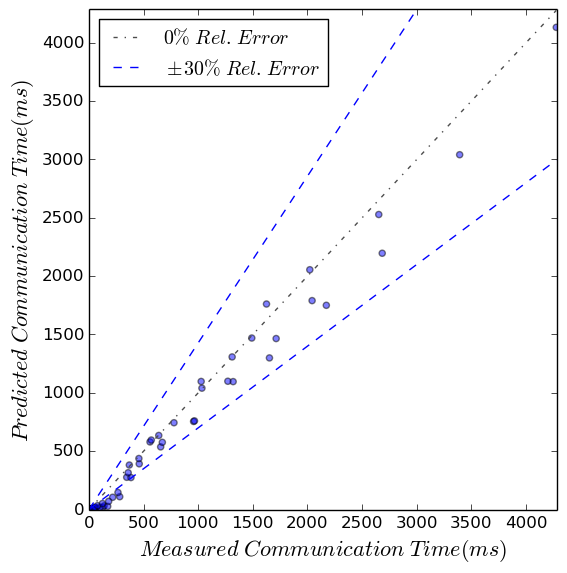
\includegraphics[width=\textwidth]{./images/NB_UMA/NB_jacobi_res.png}
        \caption{Αποτελέσματα}
        \label{fig:NB_jacobi_UMA_res}
    \end{subfigure}
    \quad %add desired spacing between images, e. g. ~, \quad, \qquad, \hfill etc. 
      %(or a blank line to force the subfigure onto a new line)
    \begin{subfigure}[b]{0.47\textwidth}
        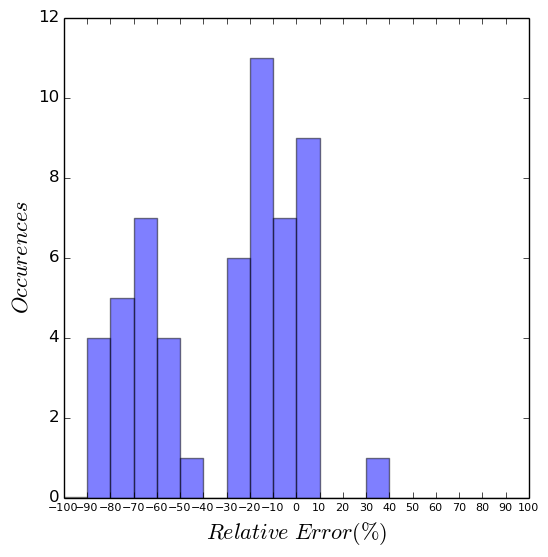
\includegraphics[width=\textwidth]{./images/NB_UMA/NB_jacobi_err_dist.png}
        \caption{Κατανομή Σφάλματος}
        \label{fig:NB_jacobi_UMA_err}
    \end{subfigure} 
    \\[0.2cm]
    \begin{subfigure}[b]{\textwidth}
   	 	\scriptsize
		\begin{tabular}{c||c|c|c|c|c}
			\textbf{Παράμετρος} & n\_estimators & learning\_rate & max\_depth & min\_samples\_leaf & min\_samples\_split \\
			\textbf{Τιμή}       &       100        &  0.1               &  8          &  3                  &    2                 
		\end{tabular}
		\caption{Παράμετροι Μοντέλου}
    \end{subfigure}
    \\[0.2cm]
    \begin{subfigure}[b]{\textwidth}
    		\centering
   	 	\scriptsize
		\begin{tabular}{c||c|c|c}
			\textbf{Μετρική} & $RCC$ &   $avg(|e|)$ & $Pred_{0.3}$  \\
			\textbf{Τιμή}  &  $0.969$   &      $33.278\%
			$        &  $60\%$                                         
		\end{tabular}
		\caption{Μετρικές Αξιολόγησης}
    \end{subfigure}
    
        \caption{Αποτελέσματα, κατανομή σφάλματος, παράμετροι εκπαίδευσης και μετρικές αξιολόγησης για την εφαρμογή Jacobi-3D σε αρχιτεκτονική UMA με το training set του p2p\_SRR}
    \label{fig:NB_jacobi_UMA}
\end{figure}
\paragraph{}
Αναλογικά με την εφαρμογή Jacobi, στο Σχήμα \ref{fig:NB_lulesh_UMA} φαίνονται τα αποτελέσματα για την εφαρμογή LULESH. Η απουσία irregular σημείων στο training set ενισχύει τις ανακρίβειες του μοντέλου για αυτή την εφαρμογή, με 6 από τα 8 χωρία να παρουσιάζουν σφάλμα μεταξύ 80-90\% και το μέσο απόλυτο σφάλμα να αγγίζει το 66.83\%.
\paragraph{}
Η μεγαλύτερη αδυναμία του training set που παράγεται από το p2p\_SRR, είναι ότι όλα τα δείγματα παράγονται μέσω ενός regular communication pattern, με αποτέλεσμα τα μοντέλα που εκπαιδεύουμε να αποτυγχάνουν να διακρίνουν τη διαφορά μεταξύ των ελάχιστων, μέσων και μέγιστων τιμών των μετρικών. Έτσι, τα χαρακτηριστικά που αφορούν ελάχιστες τιμές μετρικών έχουν ίσο ή μεγαλύτερο αντίκτυπο, ανάλογα με τον τρόπο που αναπτύσσεται το μοντέλο, στην τελική πρόβλεψη από αυτά που αντιστοιχούν σε μέσες ή μέγιστες τιμές. Το γεγονός αυτό επιδρά αρνητικά στα μοντέλα μας, καθώς, πιθανότατα, οι μετρικές αυτές, σαν ελάχιστες τιμές, έχουν ελάχιστη συσχέτιση με το χρόνο επικοινωνίας. Για να ξεπεράσουμε αυτό το εμπόδιο, έπρεπε να βρούμε τρόπο να εμπλουτίσουμε το training set που χρησιμοποιούσαμε, με σημεία στα οποία οι ελάχιστες, μέσες και μέγιστες τιμές των μετρικών διαφοροποιούνται. 

\begin{figure}[H]
    \centering
    \captionsetup{justification=centering,margin=0cm,font=footnotesize}
    \begin{subfigure}[b]{0.47\textwidth}
    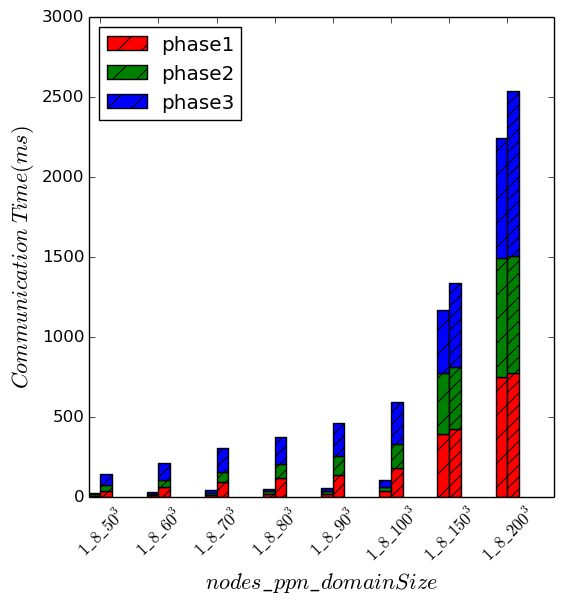
\includegraphics[width=\textwidth]{./images/NB_UMA/NB_lulesh_res.png}
    \caption{Αποτελέσματα}
    \label{fig:NB_lulesh_UMA_res}
    \end{subfigure}
    \quad %add desired spacing between images, e. g. ~, \quad, \qquad, \hfill etc. 
      %(or a blank line to force the subfigure onto a new line)
    \begin{subfigure}[b]{0.47\textwidth}
        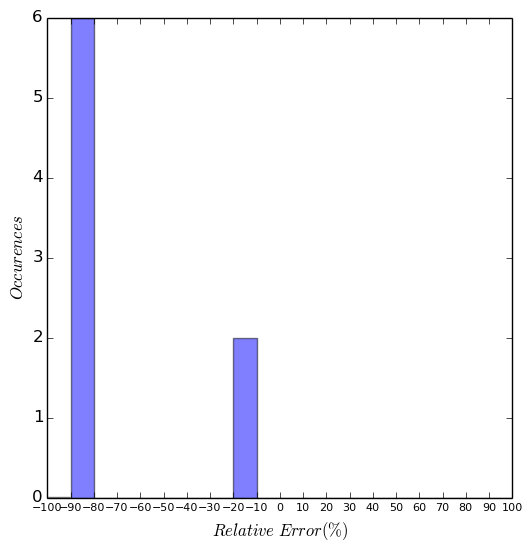
\includegraphics[width=\textwidth]{./images/NB_UMA/NB_lulesh_err_dist.png}
        \caption{Κατανομή Σφάλματος}
        \label{fig:NB_lulesh_UMA_err}
    \end{subfigure}  
    \\[0.2cm]
    \begin{subfigure}[b]{\textwidth}
   	 	\scriptsize
		\begin{tabular}{c||c|c|c|c|c}
			\textbf{Παράμετρος} & n\_estimators & learning\_rate & max\_depth & min\_samples\_leaf & min\_samples\_split \\
			\textbf{Τιμή}       &       100        &  0.1               &  8          &  3                  &    2                 
		\end{tabular}
		\caption{Παράμετροι Μοντέλου}
    \end{subfigure}
    \\[0.2cm]
    \begin{subfigure}[b]{\textwidth}
    		\centering
   	 	\scriptsize
		\begin{tabular}{c||c|c|c}
					\textbf{Μετρική} & $RCC$ &   $avg(|e|)$ & $Pred_{0.3}$  \\
			\textbf{Τιμή}  &  $1.0$   &      $66.83\%
			$        &  $0.25$                                         
		\end{tabular}
		\caption{Μετρικές Αξιολόγησης}
    \end{subfigure}
    \caption{Αποτελέσματα, κατανομή σφάλματος και παράμετροι εκπαίδευσης για την εφαρμογή LULESH σε αρχιτεκτονική UMA με το training set του p2p\_SRR. Οι λεζάντες στον οριζόντιο άξονα των αποτελεσμάτων αντιστοιχούν σε $nodes\_ppn\_$ $domainSize$.}
    \label{fig:NB_lulesh_UMA}
\end{figure}	


\subsection{Με δείγματα από τα Benchmarks p2p\_SRR και p2p\_AS}
\paragraph{}
Για να βελτιώσουμε την ακρίβεια των μοντέλων μας, δημιουργήσαμε το benchmark p2p\_AS και εντάξαμε τα δείγματα εκπαίδευσης που εξάγαμε από αυτό, σε κοινό training set με του p2p\_SRR. Σκοπός μας ήταν, με αυτά τα σημεία να δώσουμε στο μοντέλο μας παραπάνω πληροφορία για διακρίνει τις διαφορές μεταξύ των μετρικών που αποτυγχάνει να διακρίνει μόνο με τα δείγματα εκπαίδευσης του p2p\_SRR, με την εισαγωγή irregular σημείων.

\begin{figure}[ht]
    \centering
    \captionsetup{justification=centering,margin=0cm,font=footnotesize}
    \begin{subfigure}[b]{0.47\textwidth}
        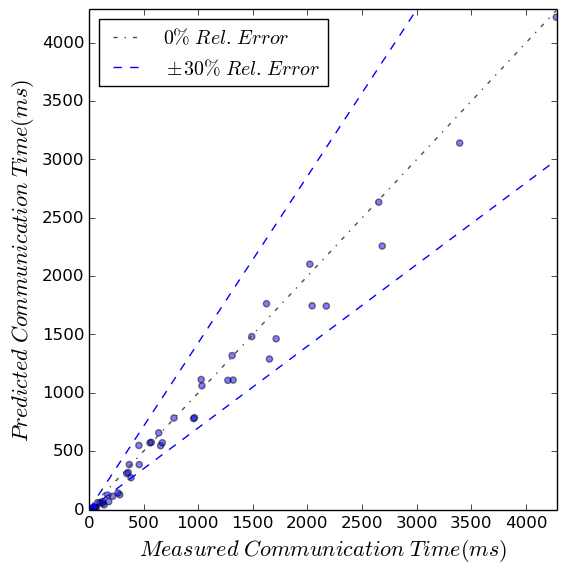
\includegraphics[width=\textwidth]{./images/NB+cg_UMA/NB_cg_jacobi_res.png}
        \caption{Αποτελέσματα}
        \label{fig:NB_cg_jacobi_UMA_res}
    \end{subfigure}
    \quad %add desired spacing between images, e. g. ~, \quad, \qquad, \hfill etc. 
      %(or a blank line to force the subfigure onto a new line)
    \begin{subfigure}[b]{0.47\textwidth}
        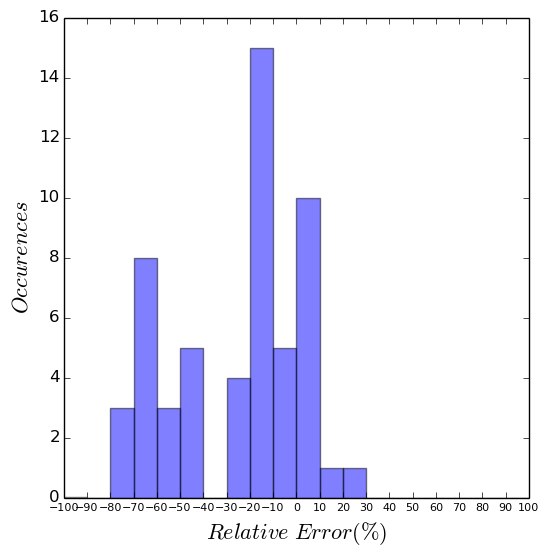
\includegraphics[width=\textwidth]{./images/NB+cg_UMA/NB_cg_jacobi_err_dist.png}
        \caption{Κατανομή Σφάλματος}
        \label{fig:NB_cg_jacobi_UMA_err}
    \end{subfigure} 
    \\[0.3cm]
    \begin{subfigure}[b]{\textwidth}
   	 	\scriptsize
		\begin{tabular}{c||c|c|c|c|c}
			\textbf{Παράμετρος} & n\_estimators & learning\_rate & max\_depth & min\_samples\_leaf & min\_samples\_split \\
			\textbf{Τιμή}       &       200        &  0.1               & 9          &  2                  &    2                 
		\end{tabular}
		\caption{Παράμετροι Μοντέλου}
    \end{subfigure}
    \\[0.3cm]
    \begin{subfigure}[b]{\textwidth}
    		\centering
   	 	\scriptsize
		\begin{tabular}{c||c|c|c}
			\textbf{Μετρική} & $RCC$ &   $avg(|e|)$ & $Pred_{0.3}$  \\
			\textbf{Τιμή}  &  $0.968$   &      $28.642\%
			$        &  $0.65$                                         
		\end{tabular}
		\caption{Μετρικές Αξιολόγησης}
    \end{subfigure}
    
        \caption{Αποτελέσματα, κατανομή σφάλματος, παράμετροι εκπαίδευσης και οι μετρικές αξιολόγησης για την εφαρμογή Jacobi-3D σε αρχιτεκτονική UMA με το training set του p2p\_SRR και του p2p\_AS. }
    \label{fig:NB+cg_jacobi_UMA}
\end{figure}
\paragraph{}
Στο Σχήμα \ref{fig:NB+cg_jacobi_UMA} φαίνονται τα αποτελέσματα, η κατανομή του σφάλματος, οι παράμετροι εκπαίδευσης του μοντέλου εκπαίδευσης και οι μετρικές αξιολόγησης για την εφαρμογή Jacobi-3D και το επεκτεταμένο training set. Παρατηρήσαμε σχετική βελτίωση στις μετρικές αξιολόγησης. Παρόλο που η τιμή του RCC παρέμενε σταθερή, το μοντέλο μας είχε 5\% μικρότερο μέσο όρο απολύτων σφαλμάτων από το προηγούμενο, ενώ τα σημεία που παρουσιάζουν σφάλμα μικρότερο από 30\% αυξάνονται στο από 60\% στο 65\% των δειγμάτων. 


\paragraph{}
Αναλογικά, στο Σχήμα \ref{fig:NB+cg_lulesh_UMA}, φαίνονται τα αντίστοιχα αποτελέσματα για την εφαρμογή LULESH. Πλέον τα σημεία που πριν αποτυγχάνουν δεν παρουσιάζουν σφάλμα 80-90\% αλλά φαίνεται ότι αντιλαμβάνονται καλύτερα τις αλλαγές στην επικοινωνία καθώς μεγαλώνουν τα χωρία της εφαρμογής. Έτσι,το μέσο απόλυτο σφάλμα μειώνεται από 66.83\% στο 53.74\%. 

\begin{figure}[ht]
    \centering
    \captionsetup{justification=centering,margin=0cm,font=footnotesize}
    \begin{subfigure}[b]{0.47\textwidth}
        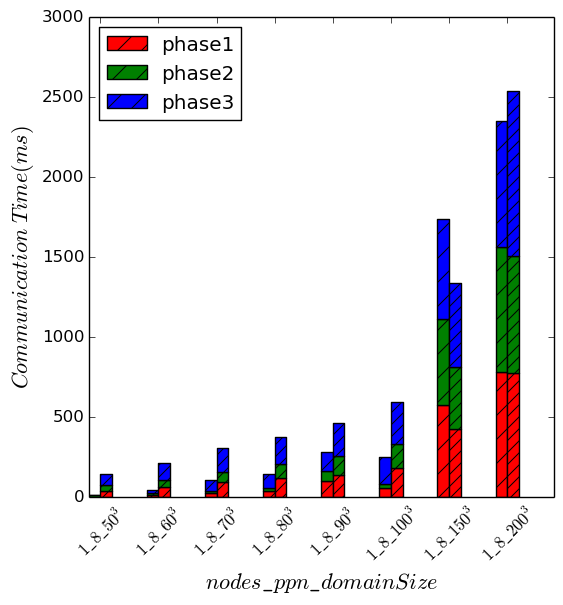
\includegraphics[width=\textwidth]{./images/NB+cg_UMA/NB_cg_lulesh_res.png}
        \caption{Αποτελέσματα}
    \end{subfigure}
    \quad %add desired spacing between images, e. g. ~, \quad, \qquad, \hfill etc. 
      %(or a blank line to force the subfigure onto a new line)
    \begin{subfigure}[b]{0.47\textwidth}
        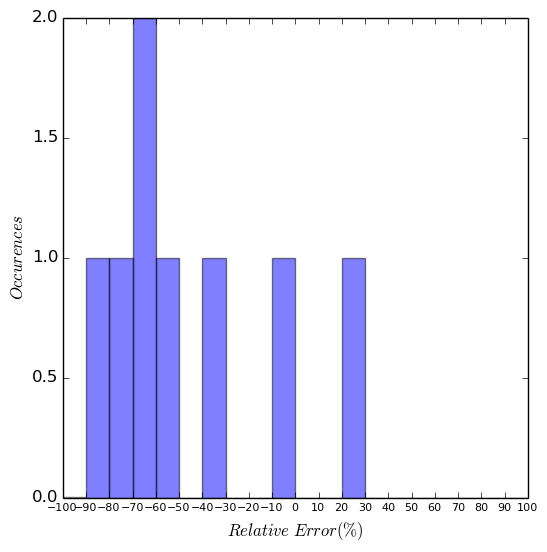
\includegraphics[width=\textwidth]{./images/NB+cg_UMA/NB_cg_lulesh_err_dist.png}
        \caption{Κατανομή Σφάλματος}
    \end{subfigure} 
    \\[0.3cm]
    \begin{subfigure}[b]{\textwidth}
   	 	\scriptsize
		\begin{tabular}{c||c|c|c|c|c}
			\textbf{Παράμετρος} & n\_estimators & learning\_rate & max\_depth & min\_samples\_leaf & min\_samples\_split \\
			\textbf{Τιμή}       &       200        &  0.1               & 9          &  2                  &    2                 
		\end{tabular}
		\caption{Παράμετροι Μοντέλου}
    \end{subfigure}
    \\[0.3cm]
    \begin{subfigure}[b]{\textwidth}
    		\centering
   	 	\scriptsize
		\begin{tabular}{c||c|c|c}
			\textbf{Μετρική} & $RCC$ &   $avg(|e|)$ & $Pred_{0.3}$  \\
			\textbf{Τιμή}  &  $0.964$   &      $53.74\%
			$        &  $25\%$                                         
		\end{tabular}
		\caption{Μετρικές Αξιολόγησης}
    \end{subfigure}
    
        \caption{Αποτελέσματα, κατανομή σφάλματος, παράμετροι εκπαίδευσης και μετρικές αξιολόγησης για την εφαρμογή LULESH σε αρχιτεκτονική UMA με το training set του p2p\_SRR και του p2p\_AS. Οι λεζάντες στον οριζόντιο άξονα των αποτελεσμάτων αντιστοιχούν σε $nodes\_ppn\_$ $domainSize$.}
    \label{fig:NB+cg_lulesh_UMA}
\end{figure}

\paragraph{}
Οφείλουμε να ομολογήσουμε ότι με την εισαγωγή των δειγμάτων από το Benchmark p2p\_AS, αναμέναμε πολύ περισσότερη βελτίωση στην ακρίβεια των μοντέλων μας από αυτή που πετύχαμε. Καταλήξαμε στο συμπέρασμα ότι τα δείγματα του p2p\_AS δεν ήταν αρκετά σε πλήθος, σε σχέση με του p2p\_SRR, για να επηρεάσουν σημαντικά τη συμπεριφορά των μοντέλων καθώς ήταν λιγότερα από το 10\% των ολικών δειγμάτων. Η εξαγωγή περαιτέρω σημείων από τη p2p\_AS κρίθηκε υπερβολικά περίπλοκη, αφού δεν είχαμε άμεση πρόσβαση στις παραμέτρους. Έτσι ακολουθήσαμε άλλες διαδικασίες. Οι περισσότερες δεν απέδωσαν ικανοποιητικά αποτελέσματα και θεωρούμε άσκοπο να τις παρουσιάσουμε. Οι πιο σημαντικές περιελάμβαναν την ανάπτυξη του benchmark p2p\_SFR, στο οποίο είχαμε τη δυνατότητα να ορίσουμε την αναλογία internode και intranode επικοινωνίας καθώς και την τυχαία απόρριψη δειγμάτων από το training set του p2p\_SRR με σκοπό την αύξηση του αντίκτυπου των δειγμάτων του p2p\_AS στο μοντέλο επικοινωνίας. Κάποιες μετρικές αξιολόγησης για αυτές τις μεθόδους δίνονται στο τέλος του κεφαλαίου.
\subsection{Με ρητή επιλογή χαρακτηριστικών}
\paragraph{}
Καθώς ούτε τα αποτελέσματα με το συνδυασμό των δειγμάτων των δύο benchmarks παρουσίαζαν ικανοποιητική επίδοση προσπαθήσαμε να παραλείψουμε χαρακτηριστικά από το training set που πιστεύαμε ότι επηρέαζαν αρνητικά τη συμπεριφορά των μοντέλων. Μετά από αρκετό πειραματισμό καταλήξαμε να κρατάμε στο training set μόνο τα χαρακτηριστικά, \textit{PPN,avgS,avgM,avgPT} και \textit{avgNT}. Τα αποτελέσματα με αυτή τη μέθοδο δίνονται στα Σχήματα \ref{fig:NB+cg_avgonly_jacobi_UMA} και \ref{fig:NB+cg_avgonly_lulesh_UMA}.

\begin{figure}[ht]
    \centering
    \captionsetup{justification=centering,margin=0cm,font=footnotesize}
    \begin{subfigure}[b]{0.47\textwidth}
        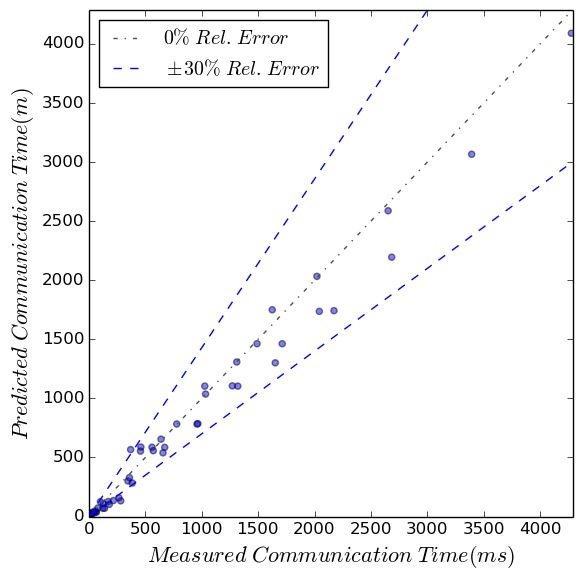
\includegraphics[width=\textwidth]{./images/NB+cg_avgonly_UMA/jacobi_res.png}
        \caption{Αποτελέσματα}
    \end{subfigure}
    \quad %add desired spacing between images, e. g. ~, \quad, \qquad, \hfill etc. 
      %(or a blank line to force the subfigure onto a new line)
    \begin{subfigure}[b]{0.47\textwidth}
        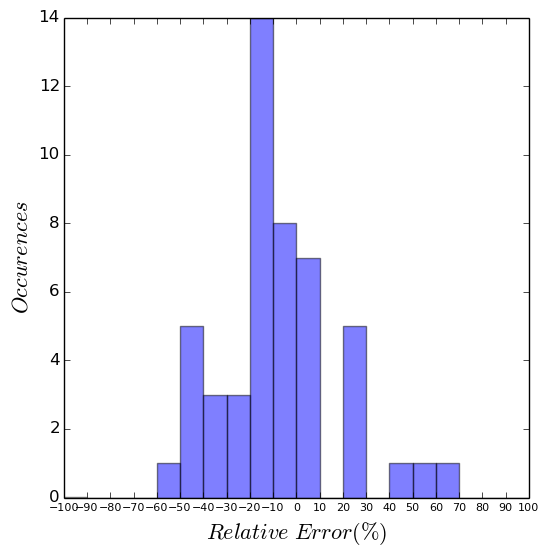
\includegraphics[width=\textwidth]{./images/NB+cg_avgonly_UMA/jacobi_err_dist.png}
        \caption{Κατανομή Σφάλματος}
    \end{subfigure} 
    \\[0.2cm]
    \begin{subfigure}[b]{\textwidth}
   	 	\scriptsize
		\begin{tabular}{c||c|c|c|c|c}
			\textbf{Παράμετρος} & n\_estimators & learning\_rate & max\_depth & min\_samples\_leaf & min\_samples\_split \\
			\textbf{Τιμή}       &       400        &  0.01               & 8          &  3                  &    3                 
		\end{tabular}
		\caption{Παράμετροι Μοντέλου}
    \end{subfigure}
    \\[0.2cm]
    \begin{subfigure}[b]{\textwidth}
    		\centering
   	 	\scriptsize
		\begin{tabular}{c||c|c|c}
			\textbf{Μετρική} & $RCC$ &   $avg(|e|)$ & $Pred_{0.3}$  \\
			\textbf{Τιμή}  &  $0.964$   &      $22.6\%
			$        &  $74\%$                                         
		\end{tabular}
		\caption{Μετρικές Αξιολόγησης}
    \end{subfigure}
    
        \caption{Αποτελέσματα, κατανομή σφάλματος, παράμετροι εκπαίδευσης και μετρικές αξιολόγησης για την εφαρμογή Jacobi-3D σε αρχιτεκτονική UMA με ρητή επιλογή παραμέτρων}
    \label{fig:NB+cg_avgonly_jacobi_UMA}
\end{figure}

\begin{figure}[H]
    \centering
    \captionsetup{justification=centering,margin=0cm,font=footnotesize}
    \begin{subfigure}[b]{0.47\textwidth}
        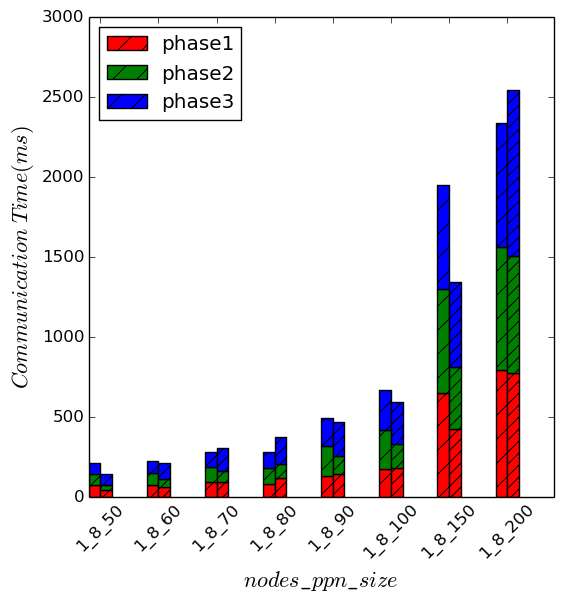
\includegraphics[width=\textwidth]{./images/NB+cg_avgonly_UMA/lulesh_res.png}
        \caption{Αποτελέσματα}
    \end{subfigure}
    \quad %add desired spacing between images, e. g. ~, \quad, \qquad, \hfill etc. 
      %(or a blank line to force the subfigure onto a new line)
    \begin{subfigure}[b]{0.47\textwidth}
        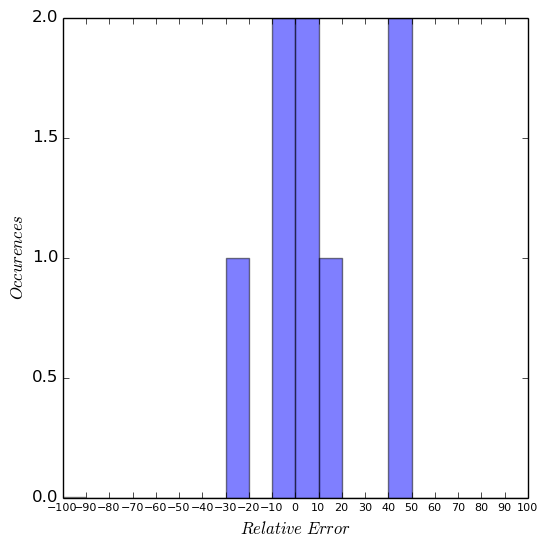
\includegraphics[width=\textwidth]{./images/NB+cg_avgonly_UMA/lulesh_err_dist.png}
        \caption{Κατανομή Σφάλματος}
    \end{subfigure} 
    \\[0.2cm]
    \begin{subfigure}[b]{\textwidth}
   	 	\scriptsize
		\begin{tabular}{c||c|c|c|c|c}
			\textbf{Παράμετρος} & n\_estimators & learning\_rate & max\_depth & min\_samples\_leaf & min\_samples\_split \\
			\textbf{Τιμή}       &       400        &  0.007               & 10          &  1                  &    3                 
		\end{tabular}
		\caption{Παράμετροι Μοντέλου}
    \end{subfigure}
    \\[0.2cm]
    \begin{subfigure}[b]{\textwidth}
    		\centering
   	 	\scriptsize
		\begin{tabular}{c||c|c|c}
			\textbf{Μετρική} & $RCC$ &   $avg(|e|)$ & $Pred_{0.3}$  \\
			\textbf{Τιμή}  &  $0.964$   &      $19.450\%
			$        &  $75\%$                                         
		\end{tabular}
		\caption{Μετρικές Αξιολόγησης}
    \end{subfigure}
    
        \caption{Αποτελέσματα, κατανομή σφάλματος, παράμετροι εκπαίδευσης και μετρικές αξιολόγησης για την εφαρμογή LULESH σε αρχιτεκτονική UMA με ρητή επιλογή παραμέτρων. Οι λεζάντες στον οριζόντιο άξονα των αποτελεσμάτων αντιστοιχούν σε $nodes\_ppn\_domainSize$.}
    \label{fig:NB+cg_avgonly_lulesh_UMA}
\end{figure}

\paragraph{}
Η βελτίωση στα αποτελέσματα είναι προφανής. Για την εφαρμογή Jacobi-3D, το μέσο απόλυτο σφάλμα μειώνεται από 28\% στο 22\%. ενώ περίπου τρία τέταρτα των προβλέψεων παρουσιάζουν σφάλμα μικρότερο από 30\% διατηρώντας ψηλή τιμή για το RCC. Επιπρόσθετα, η εφαρμογή LULESH παρουσίασε τη μεγαλύτερη βελτίωση με την παράλειψη κάποιων μετρικών. Οι μετρικές που κρατήσαμε ήταν οι ίδιες με την εφαρμογή Jacobi-3D. Το μέσο απόλυτο σφάλμα μειώθηκε κατά 34\% με την νέα τιμή να περιοριζόταν στο 19.5\%  ενώ 75\% των προβλέψεων πέτυχαν σφάλμα μικρότερο του 20\%. Αυτές οι προβλέψεις ήταν και οι καλύτερες που καταφέραμε να πετύχουμε.





\section{Αποτελέσματα για την αρχιτεκτονική NUMA}

\paragraph{}
Σε επόμενο στάδιο, αναφερόμαστε στα αποτελέσματα της μεθοδολογίας μας για την αρχιτεκτονική NUMA. Καθώς πλέον λαμβάνει χώρα internode και intranode επικοινωνία ταυτόχρονα, στη γενική περίπτωση όλες οι μετρικές έχουν μη μηδενικές τιμές. Σαν αποτέλεσμα, κάναμε χρήση αλγορίθμων επιλογής χαρακτηριστικών (feature selection) για να αφαιρέσουμε από το training set μετρικές οι οποίες απλά εισήγαγαν θόρυβο και αχρείαστη πληροφορία στο μοντέλο. Η ροή με την οποία παρουσιάζονται τα αποτελέσματα είναι η ίδια με την αρχιτεκτονική UMA, με τα βήματα που ακολουθήσαμε για να καταλήξουμε στα καλύτερα αποτελέσματα. 

\subsection{Με δείγματα από το benchmark p2p\_SRR}
Η πρώτη μας προσπάθεια αφορά τα αποτελέσματα με το training set που εξάγαμε από το benchmark p2p\_SRR. Στα Σχήματα \ref{fig:NB_jacobi_NUMA} και \ref{fig:NB_lulesh_NUMA} παραθέτουμε τα αποτελέσματα για τις δύο εφαρμογές.

\begin{figure}
    \centering
    \captionsetup{justification=centering,margin=0cm,font=footnotesize}
    \begin{subfigure}[b]{0.47\textwidth}
        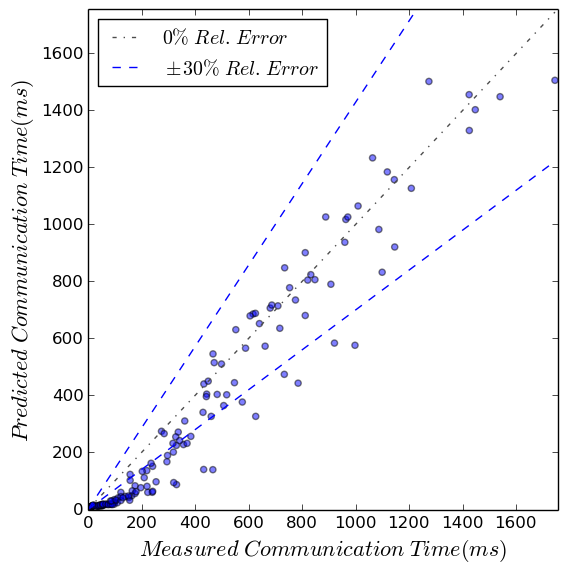
\includegraphics[width=\textwidth]{./images/NB_NUMA/jacobi_res_nfe.png}
        \caption{Αποτελέσματα}
    \end{subfigure}
    \quad %add desired spacing between images, e. g. ~, \quad, \qquad, \hfill etc. 
      %(or a blank line to force the subfigure onto a new line)
    \begin{subfigure}[b]{0.47\textwidth}
        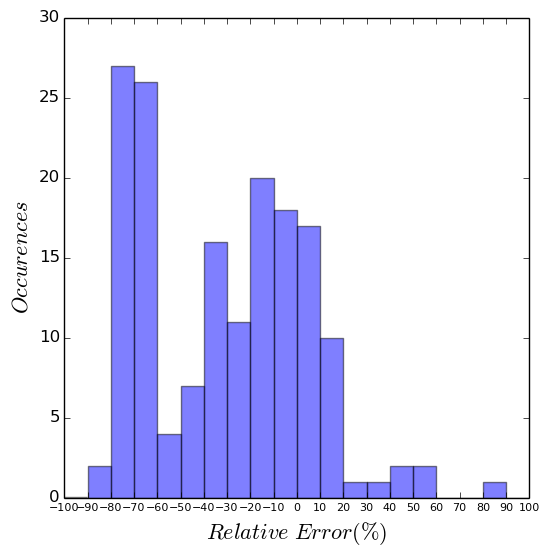
\includegraphics[width=\textwidth]{./images/NB_NUMA/jacobi_err_dist_nfe.png}
        \caption{Κατανομή Σφάλματος}
    \end{subfigure} 
    \\[0.2cm]
    \begin{subfigure}[b]{\textwidth}
   	 	\scriptsize
		\begin{tabular}{c||c|c|c|c|c}
			\textbf{Παράμετρος} & n\_estimators & learning\_rate & max\_depth & min\_samples\_leaf & min\_samples\_split \\
			\textbf{Τιμή}       &       1000        &  0.1               & 10          &  4                  &    2
		\end{tabular}
		\caption{Παράμετροι Μοντέλου}
    \end{subfigure}
    \\[0.2cm]
    \begin{subfigure}[b]{\textwidth}
    		\centering
   	 	\scriptsize
		\begin{tabular}{c||c|c|c}
			\textbf{Μετρική} & $RCC$ &   $avg(|e|)$ & $Pred_{0.3}$  \\
			\textbf{Τιμή}  &  $0.953$   &      $37.398\%
			$        &  $47\%$                                         
		\end{tabular}
		\caption{Μετρικές Αξιολόγησης}
    \end{subfigure}
    
        \caption{Αποτελέσματα, κατανομή σφάλματος, παράμετροι εκπαίδευσης και μετρικές αξιολόγησης για την εφαρμογή Jacobi σε αρχιτεκτονική NUMA με το Benchmark p2p\_SRR}
    \label{fig:NB_jacobi_NUMA}
\end{figure}
\begin{figure}
    \centering
    \captionsetup{justification=centering,margin=0cm,font=footnotesize}
    \begin{subfigure}[b]{0.47\textwidth}
        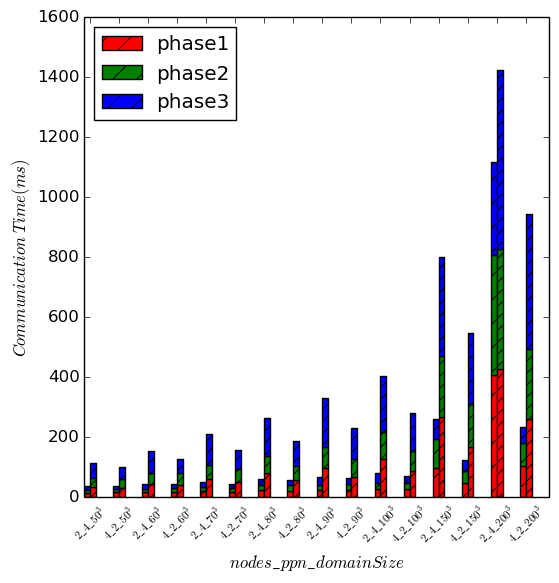
\includegraphics[width=\textwidth]{./images/NB_NUMA/lulesh_res_nfe.png}
        \caption{Αποτελέσματα}
    \end{subfigure}
    \quad %add desired spacing between images, e. g. ~, \quad, \qquad, \hfill etc. 
      %(or a blank line to force the subfigure onto a new line)
    \begin{subfigure}[b]{0.47\textwidth}
        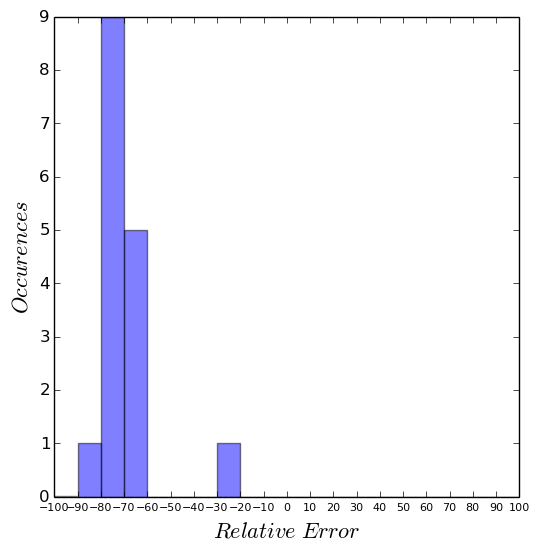
\includegraphics[width=\textwidth]{./images/NB_NUMA/lulesh_err_dist_nfe.png}
        \caption{Κατανομή Σφάλματος}
    \end{subfigure} 
    \\[0.2cm]
    \begin{subfigure}[b]{\textwidth}
   	 	\scriptsize
		\begin{tabular}{c||c|c|c|c|c}
			\textbf{Παράμετρος} & n\_estimators & learning\_rate & max\_depth & min\_samples\_leaf & min\_samples\_split \\
			\textbf{Τιμή}       &       1000        &  0.1               & 10          &  4                  &    2
		\end{tabular}
		\caption{Παράμετροι Μοντέλου}
    \end{subfigure}
    \\[0.2cm]
    \begin{subfigure}[b]{\textwidth}
    		\centering
   	 	\scriptsize
		\begin{tabular}{c||c|c|c}
			\textbf{Μετρική} & $RCC$ &   $avg(|e|)$ & $Pred_{0.3}$  \\
			\textbf{Τιμή}  &  $0.958$   &      $69.42\%
			$        &  $6\%$                                         
		\end{tabular}
		\caption{Μετρικές Αξιολόγησης}
    \end{subfigure}
    
        \caption{Αποτελέσματα, κατανομή σφάλματος, παράμετροι εκπαίδευσης και μετρικές αξιολόγησης για την εφαρμογή LULESH σε αρχιτεκτονική NUMA με το Benchmark p2p\_SRR}
    \label{fig:NB_lulesh_NUMA}
\end{figure}
\paragraph{}
Δυστυχώς, η πρώτη μας προσπάθεια δεν παρουσίαζε ιδιαίτερη ακρίβεια. Αναφορικά με την εφαρμογή Jacobi-3D, μόλις 47\% των προβλέψεων πετύχαιναν απόλυτο σφάλμα μικρότερο του 30\% ενώ το μέσο απόλυτο σφάλμα άγγιζε το 37.4\%. Επιπλέον, 54 από τα 176 δείγματα, παρουσίαζαν σφάλμα 60\% με 80\% με τις προβλέψεις να είναι σημαντικά μικρότερες από τις μετρούμενες τιμές. Επιπλέον, τα αποτελέσματα ήταν απογοητευτικά για την εφαρμογή LULESH, με μόλις μία από τις δεκαέξι προβλέψεις να έχει σφάλμα μικρότερο του 30\% και το μέσω σφάλμα να είναι κοντά στο 70\%. Προσπαθήσαμε να βελτιώσουμε τις προβλέψεις με χρήση μεθόδων feature selection χωρίς ιδιαίτερη επιτυχία, έτσι δεν θα παρουσιάσουμε τα αποτελέσματα τους.

\paragraph{} 
Καταλήψαμε στο συμπέρασμα ότι η ανακρίβεια με τα σημεία εκπαίδευσης του bench\-mark p2p\_SRR οφείλεται σε δύο λόγους. Ο πρώτος, με το μεγάλυτερο αντίκτυπο στις προβλέψεις του LULESH, είναι ξανά η απουσία irregular σημείων από το σύνολο εκπαίδευσης. Ο δεύτερος, αφορά την αναλογία internode και intranode επικοινωνίας που καταλήγουν να εμφανίζουν τα σημεία. Όπως αναφέραμε, στο benchmark p2p\_SRR κάθε διεργασία, επιλέγει τυχαία κάποια άλλη για την ανταλλαγή δεδομένων για κάθε μήνυμα ξεχωριστά. Ωστόσο, η επιλογή αυτή είναι μεν τυχαία αλλά υπάρχει μεγαλύτερη πιθανότητα να επιλεγεί διεργασία για ανταλλαγή, που βρίσκεται σε άλλο κόμβο αφού οι διεργασίες αυτές είναι περισσότερες σε αριθμό. Έτσι, η αναλογία internode και intranode επικοινωνίας σύγκλινε περίπου στο 75\% υπέρ της internode επικοινωνίας ανάλογα πάντα και με το PPN. Αυτός ήταν και ο κύριος λόγος που αναπτύξαμε το benchmark p2p\_SFR που μας έδινε την δυνατότητα να ορίζουμε το επιθυμητό ratio μεταξύ των δύο τύπων επικοινωνίας. Παρόλα αυτά, δεν είχαμε την ανάλογη βελτίωση στα αποτελέσματα.

\subsection{Με δείγματα από τα benchmark p2p\_SRR και p2p\_AS}
\paragraph{}
Μετέπειτα εντάξαμε τα δείγματα από το benchmark p2p\_AS, σε κοινό training set με το p2p\_SRR ακολουθώντας την ίδια συλλογιστική με την UMA αρχιτεκτονική. Εκπαιδεύσαμε μοντέλα με και χωρίς feature selection μεθόδους. Με την ένταξη των σημείων του p2p\_AS στο training set, τα μοντέλα με feature selection παρουσίαζαν μεγαλύτερη ακρίβεια ενώ απαιτούσαν λιγότερο χρόνο για την εκπαίδευσή τους. Τα σχετικά γραφήματα για τις δύο εφαρμογές με feature selection φαίνονται στα Σχήματα \ref{fig:NB_cg_jacobi_NUMA} και \ref{fig:NB_cg_lulesh_NUMA}. Επιπλέον στο Σχήμα \ref{fig:NB_cg_importances} δίνονται τα χαρακτηριστικά που δεν απορρίφθηκαν  και τα αντίστοιχα importances τους στη τελική πρόβλεψη.

\paragraph{}
Από τις γραφικές φαίνεται βελτίωση στη συμπεριφορά των μοντέλων και για τις δύο εφαρμογές. Συγκεκριμένα, αναφορικά με τις μετρικές αξιολόγησης, πετύχαμε 12\% μείωση στο μέσο απόλυτο σφάλμα και αύξηση του $Pred_{0.3}$ στο 67\% για την εφαρμογή Jacobi-3D. Οι προβλέψεις για την εφαρμογή LULESH παρουσιάζουν τεράστια βελτίωση, με το μέσο σφάλμα να μειώνεται κατά 33\% και το $Pred_{0.3}$ αυξάνεται κατά 25\%. Ωστόσο, αποκλίνουν και πάλι αρκετά από τις μετρούμενες τιμές, με μέσο σφάλμα 36.6\%. Από τα importances, παρατηρήσαμε ότι τα πιο σημαντικά χαρακτηριστικά ήταν αυτά που υπολογίζονταν από την κίνηση δεδομένων μεταξύ των κόμβων. Παρόλο που περιμέναμε διαφορές μεταξύ των ελάχιστων, μέσων και μέγιστων χαρακτηριστικών αναμέναμε ότι σε κάθε περίπτωση οι ελάχιστες τιμές θα είχαν ελάχιστο αντίκτυπο στη πρόβλεψη. Ο λόγος που αυτό δεν επιτυγχάνεται, είναι ο ίδιος με την UMA αρχιτεκτονική . Τα δείγματα προερχόμενα από regular communication patterns είναι χιλιάδες, ενώ από irregular εκατοντάδες. Έτσι, η επίδραση τους στο μοντέλο επικοινωνίας είναι περιορισμένη.

\begin{figure}[ht]
    \centering
    \captionsetup{justification=centering,margin=0cm,font=footnotesize}
    \begin{subfigure}[b]{0.47\textwidth}
        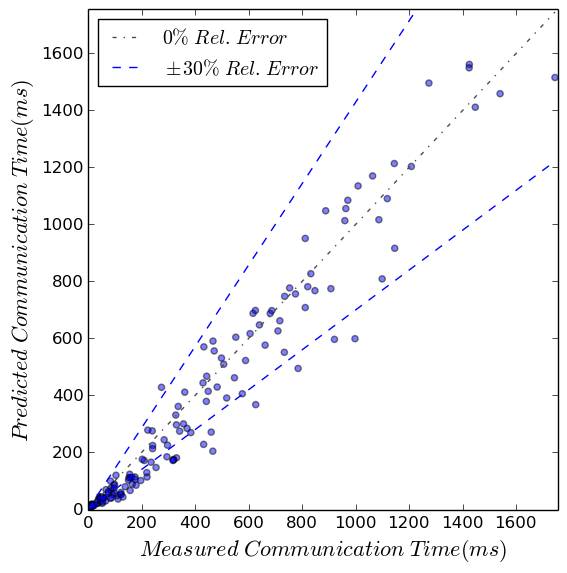
\includegraphics[width=\textwidth]{./images/NB+cg_NUMA/NB_cg_jacobi_res.png}
        \caption{Αποτελέσματα}
    \end{subfigure}
    \quad %add desired spacing between images, e. g. ~, \quad, \qquad, \hfill etc. 
      %(or a blank line to force the subfigure onto a new line)
    \begin{subfigure}[b]{0.47\textwidth}
        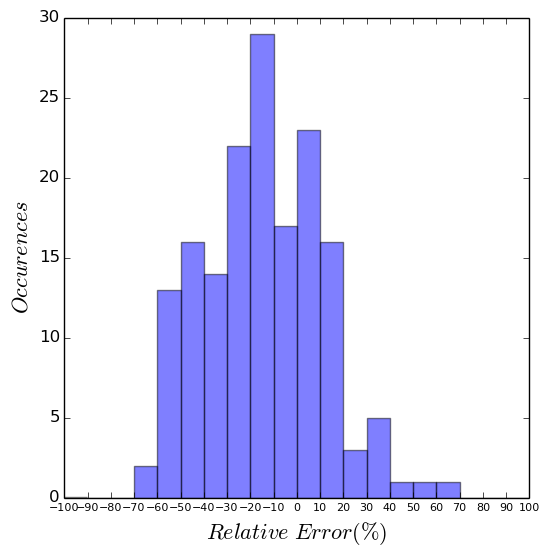
\includegraphics[width=\textwidth]{./images/NB+cg_NUMA/NB_cg_jacobi_err_dist.png}
        \caption{Κατανομή Σφάλματος}
    \end{subfigure} 
    \\[0.2cm]
    \begin{subfigure}[b]{\textwidth}
   	 	\scriptsize
		\begin{tabular}{c||c|c|c|c|c}
			\textbf{Παράμετρος} & n\_estimators & learning\_rate & max\_depth & min\_samples\_leaf & min\_samples\_split \\
			\textbf{Τιμή}       &       2000        &  0.1               & 12          &  3                  &    2
		\end{tabular}
		\caption{Παράμετροι Μοντέλου}
    \end{subfigure}
    \\[0.2cm]
    \begin{subfigure}[b]{\textwidth}
    		\centering
   	 	\scriptsize
		\begin{tabular}{c||c|c|c}
			\textbf{Μετρική} & $RCC$ &   $avg(|e|)$ & $Pred_{0.3}$  \\
			\textbf{Τιμή}  &  $0.947$   &      $25.15\%
			$        &  $67\%$                                         
		\end{tabular}
		\caption{Μετρικές Αξιολόγησης}
    \end{subfigure}
    
        \caption{Αποτελέσματα, κατανομή σφάλματος, παράμετροι εκπαίδευσης και μετρικές αξιολόγησης για την εφαρμογή Jacobi σε αρχιτεκτονική NUMA με τα Benchmarks p2p\_SRR και p2p\_AS}
    \label{fig:NB_cg_jacobi_NUMA}
\end{figure}
\begin{figure}[ht]
    \centering
    \captionsetup{justification=centering,margin=0cm,font=footnotesize}
    \begin{subfigure}[b]{0.47\textwidth}
        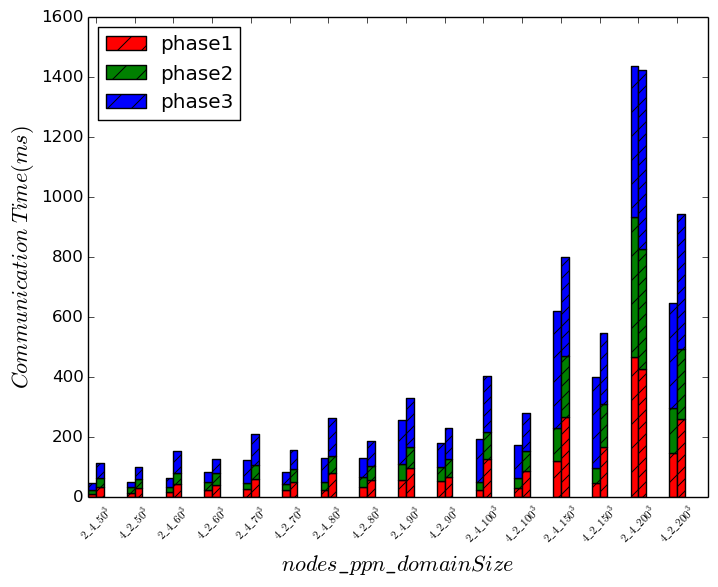
\includegraphics[width=\textwidth]{./images/NB+cg_NUMA/NB_cg_lulesh_res.png}
        \caption{Αποτελέσματα}
    \end{subfigure}
    \quad %add desired spacing between images, e. g. ~, \quad, \qquad, \hfill etc. 
      %(or a blank line to force the subfigure onto a new line)
    \begin{subfigure}[b]{0.47\textwidth}
        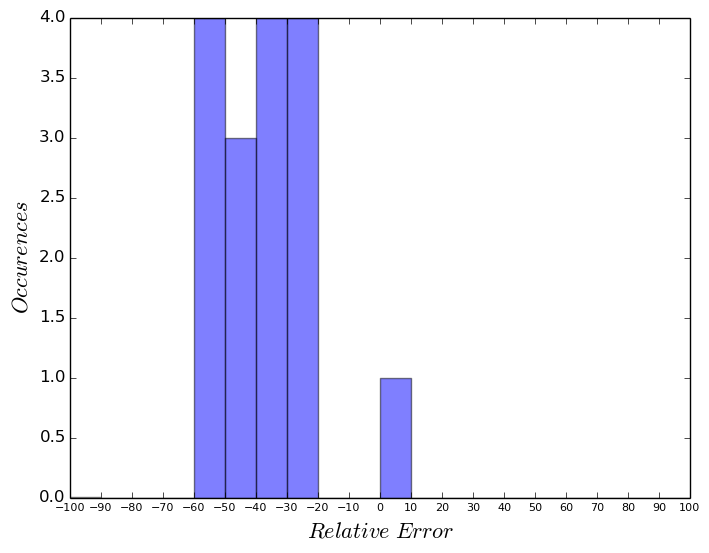
\includegraphics[width=\textwidth]{./images/NB+cg_NUMA/NB_cg_lulesh_err_dist.png}
        \caption{Κατανομή Σφάλματος}
    \end{subfigure} 
    \\[0.2cm]
    \begin{subfigure}[b]{\textwidth}
   	 	\scriptsize
		\begin{tabular}{c||c|c|c|c|c}
			\textbf{Παράμετρος} & n\_estimators & learning\_rate & max\_depth & min\_samples\_leaf & min\_samples\_split \\
			\textbf{Τιμή}       &       2000        &  0.1               & 12          &  3                  &    2
		\end{tabular}
		\caption{Παράμετροι Μοντέλου}
    \end{subfigure}
    \\[0.2cm]
    \begin{subfigure}[b]{\textwidth}
    		\centering
   	 	\scriptsize
		\begin{tabular}{c||c|c|c}
			\textbf{Μετρική} & $RCC$ &   $avg(|e|)$ & $Pred_{0.3}$  \\
			\textbf{Τιμή}  &  $0.950$   &      $36.60\%
			$        &  $31\%$                                         
		\end{tabular}
		\caption{Μετρικές Αξιολόγησης}
    \end{subfigure}
    
        \caption{Αποτελέσματα, κατανομή σφάλματος, παράμετροι εκπαίδευσης και μετρικές αξιολόγησης για την εφαρμογή LULESH σε αρχιτεκτονική NUMA με τα Benchmarks p2p\_SRR και p2p\_AS. Οι λεζάντες στον οριζόντιο άξονα των αποτελεσμάτων αντιστοιχούν σε $nodes\_ppn\_domainSize$.}
    \label{fig:NB_cg_lulesh_NUMA}
\end{figure}

\begin{figure}[H]
    \centering
    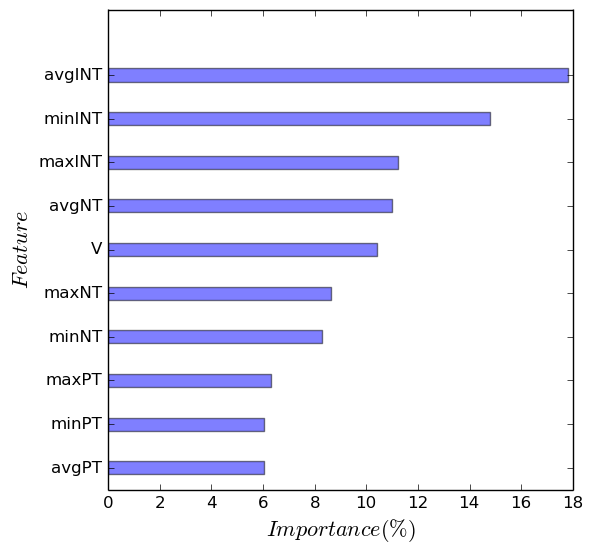
\includegraphics[width=0.7\textwidth]{./images/importance_manually.png}
    \caption{Εναπομείναντα χαρακτηριστικά και τα importances τους}
    \label{fig:NB_cg_importances}
\end{figure}


\subsection{Με ρητή επιλογή χαρακτηριστικών}
\paragraph{}
Καθώς θέλαμε να αυξήσουμε τον αντίκτυπο του \textit{p2p\_AS} στις προβλέψεις, αποφασίσαμε να κάνουμε ρητή επιλογή χαρακτηριστικών με βάση τη διάταξη των importances για ένα μοντέλο εκπαιδευμένο μόνο με το training set του p2p\_AS. Χρησιμοποιώντας τα αποτελέσματα, επιλέγαμε τις μετρικές που θα διατηρούσαμε στο τελικό training set, που περιείχε δείγματα και από τα δύο benchmarks. Στο Σχήμα \ref{fig:importances} δίνονται τα importances για τα δύο training sets. Όπως φαίνεται από στο σχήμα, υπάρχουν σημαντικές διαφορές στην επιρροή των χαρακτηριστικών στην τελική πρόβλεψη. Έτσι, επιβεβαιώνεται ο ισχυρισμός μας, για την αδυναμία του p2p\_AS training set να επηρεάσει το μεγάλο, κοινό training set.

\begin{figure}[ht]
    \centering
    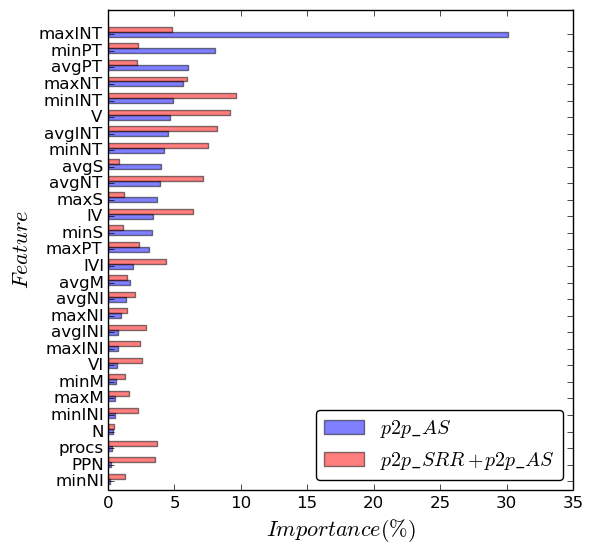
\includegraphics[width=0.7\textwidth]{./images/importance.png}
    \caption{Importances για τα δύο training sets}
    \label{fig:importances}
\end{figure}

\paragraph{}
Οι πιο μεγάλες διαφορές ανάμεσα στα importances αφορούν τις μετρικές NT και ΙΝΤ. Στο p2p\_SRR+p2p\_AS, το minINT είναι το χαρακτηριστικό με το μεγαλύτερο αντίκτυπο στο τελικό αποτέλεσμα. Αντίθετα, στο p2p\_AS, πιο σημαντικό χαρακτηριστικό είναι το maxINT, που αποτελεί διαισθητικά καλύτερη επιλογή καθώς αναμέναμε ότι ο περισσότερος χρόνος επικοινωνίας αναλώνεται για την internode επικοινωνία της εφαρμογής. Επιπρόσθετα, αναφορικά με την INT μετρική, παρατηρούμε μείωση στο importance της ελάχιστης και μέσης τιμής, με τη μέγιστη να μένει αμετάβλητη. Τα χαρακτηριστικά που αφορούν Injection και παραμέτρους εκτέλεσης της εφαρμογής δεν φαίνεται να έχουν ιδιαίτερη επίδραση στο τελικό χρόνο επικοινωνίας με αποτέλεσμα να μην περιλαμβάνονται καθόλου στο τελικό training set, ενώ η μετρική PT είναι η μόνη που διατηρεί την προβληματική συμπεριφορά, με την ελάχιστη τιμή της να έχει μεγαλύτερη σημασία από την μέγιστη.

\paragraph{}
Τα τελικά χαρακτηριστικά που περιλήφθηκαν στο training set ήταν τα $maxS$, $maxPT$, $maxNT$, $maxINT$, $V$ και $IV$. Αποφασίσαμε να αψηφήσουμε το ranking των χαρακτηριστικών για το PT και να συμπεριλάβουμε την μέγιστη τιμή του αντί της ελάχιστης. Τα αναλυτικά αποτελέσματα και για τις δύο εφαρμογές δίνονται στα Σχήματα \ref{fig:NB_cg_mfs_jacobi_NUMA} και \ref{fig:NB_cg_mfs_lulesh_NUMA}
\begin{figure}[ht]
    \centering
    \captionsetup{justification=centering,margin=0cm,font=footnotesize}
    \begin{subfigure}[b]{0.47\textwidth}
        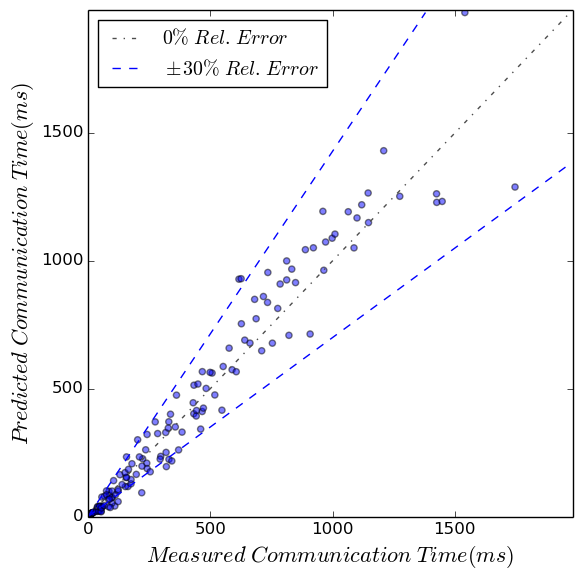
\includegraphics[width=\textwidth]{./images/NB+cg_mfs_NUMA/jacobi_res.png}
        \caption{Αποτελέσματα}
    \end{subfigure}
    \quad %add desired spacing between images, e. g. ~, \quad, \qquad, \hfill etc. 
      %(or a blank line to force the subfigure onto a new line)
    \begin{subfigure}[b]{0.47\textwidth}
        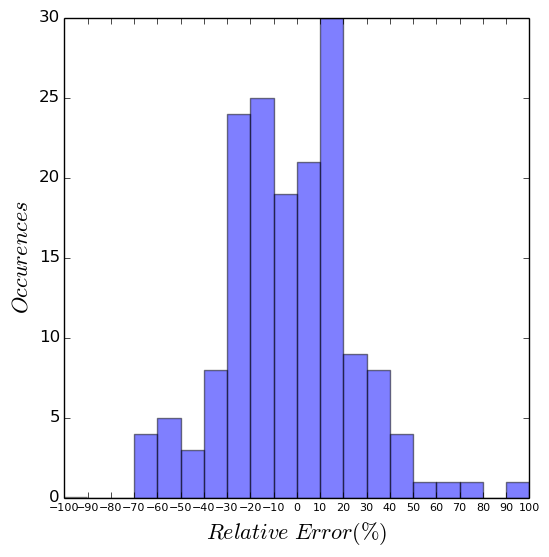
\includegraphics[width=\textwidth]{./images/NB+cg_mfs_NUMA/jacobi_err_dist.png}
        \caption{Κατανομή Σφάλματος}
    \end{subfigure} 
    \\[0.2cm]
    \begin{subfigure}[b]{\textwidth}
   	 	\scriptsize
		\begin{tabular}{c||c|c|c|c|c}
			\textbf{Παράμετρος} & n\_estimators & learning\_rate & max\_depth & min\_samples\_leaf & min\_samples\_split \\
			\textbf{Τιμή}       &       2000        &  0.005          & 10          &  4                  &    5
		\end{tabular}
		\caption{Παράμετροι Μοντέλου}
    \end{subfigure}
    \\[0.2cm]
    \begin{subfigure}[b]{\textwidth}
    		\centering
   	 	\scriptsize
		\begin{tabular}{c||c|c|c}
			\textbf{Μετρική} & $RCC$ &   $avg(|e|)$ & $Pred_{0.3}$  \\
			\textbf{Τιμή}  &  $0.956$   &      $22.116\%
			$        &  $78\%$                                         
		\end{tabular}
		\caption{Μετρικές Αξιολόγησης}
    \end{subfigure}
    
        \caption{Αποτελέσματα, κατανομή σφάλματος, παράμετροι εκπαίδευσης και μετρικές αξιολόγησης για την εφαρμογή Jacobi σε αρχιτεκτονική NUMA με ρητή επιλογή παραμέτρων.}
    \label{fig:NB_cg_mfs_jacobi_NUMA}
\end{figure}
\begin{figure}[H]
    \centering
    \captionsetup{justification=centering,margin=0cm,font=footnotesize}
    \begin{subfigure}[b]{0.47\textwidth}
        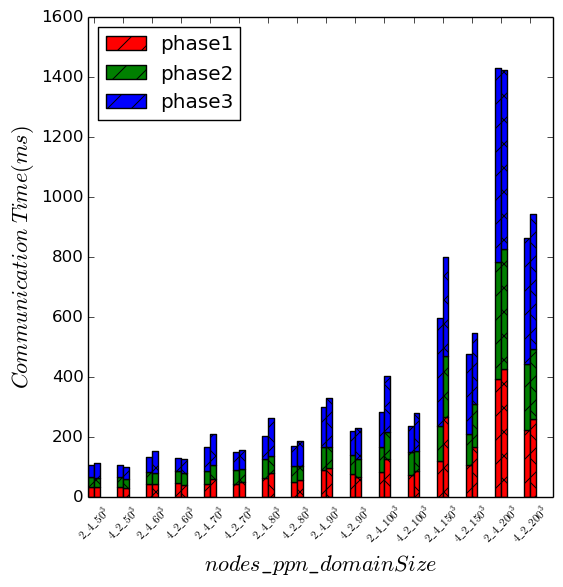
\includegraphics[width=\textwidth]{./images/NB+cg_mfs_NUMA/lulesh_res.png}
        \caption{Αποτελέσματα}
    \end{subfigure}
    \quad %add desired spacing between images, e. g. ~, \quad, \qquad, \hfill etc. 
      %(or a blank line to force the subfigure onto a new line)
    \begin{subfigure}[b]{0.47\textwidth}
        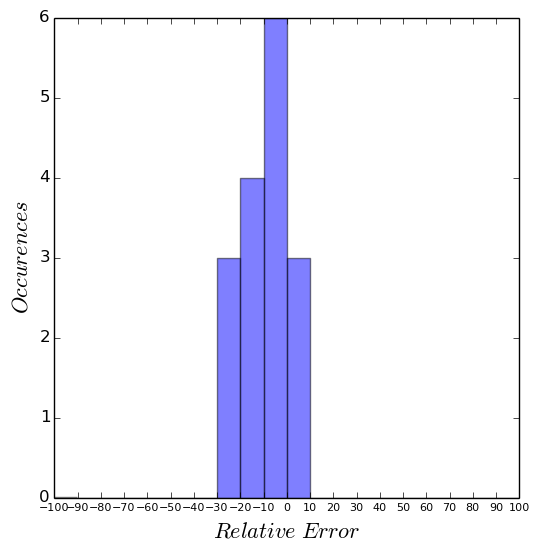
\includegraphics[width=\textwidth]{./images/NB+cg_mfs_NUMA/lulesh_err_dist.png}
        \caption{Κατανομή Σφάλματος}
    \end{subfigure} 
    \\[0.2cm]
    \begin{subfigure}[b]{\textwidth}
   	 	\scriptsize
		\begin{tabular}{c||c|c|c|c|c}
			\textbf{Παράμετρος} & n\_estimators & learning\_rate & max\_depth & min\_samples\_leaf & min\_samples\_split \\
			\textbf{Τιμή}       &       2000        &  0.002               & 10          &  4                  &    5
		\end{tabular}
		\caption{Παράμετροι Μοντέλου}
    \end{subfigure}
    \\[0.2cm]
    \begin{subfigure}[b]{\textwidth}
    		\centering
   	 	\scriptsize
		\begin{tabular}{c||c|c|c}
			\textbf{Μετρική} & $RCC$ &   $avg(|e|)$ & $Pred_{0.3}$  \\
			\textbf{Τιμή}  &  $0.975$   &      $12.05\%
			$        &  $100\%$                                         
		\end{tabular}
		\caption{Μετρικές Αξιολόγησης}
    \end{subfigure}
    
        \caption{Αποτελέσματα, κατανομή σφάλματος, παράμετροι εκπαίδευσης και μετρικές αξιολόγησης για την εφαρμογή LULESH σε αρχιτεκτονική NUMA με ρητή επιλογή παραμέτρων. Οι λεζάντες στον οριζόντιο άξονα των αποτελεσμάτων αντιστοιχούν σε $nodes\_ppn\_domainSize$.}
    \label{fig:NB_cg_mfs_lulesh_NUMA}
\end{figure}

\paragraph{}
Η ακρίβεια και η συμπεριφορά των τελευταίων μοντέλων ξεπερνά όλες τις προηγούμενές μας προσπάθειες. Για την εφαρμογή Jacobi, καταφέραμε να βελτιώσουμε όλες τις μετρικές αξιολόγησης με σχεδόν 80\% των προβλέψεων να παρουσιάζουν απόλυτο σφάλμα μικρότερο από 30\%. Επιπρόσθετα, μεγάλη βελτίωση παρουσιάζεται για την εφαρμογή LULESH. Το μέσο απόλυτο σφάλμα μειώνεται από 36.6\% στο 12.05\% με όλες τις προβλέψεις να παρουσιάζουν απόλυτο σφάλμα μικρότερο από 30\%. Σ' αυτό το σημείο, θεωρήσαμε ότι περαιτέρω βελτίωση της μεθοδολογίας δεν ήταν απαραίτητη.

\section{Συνολική Αξιολόγηση}
\paragraph{}
Στους Πίνακες \ref{table:metrics_jacobi} και \ref{table:metrics_lulesh} δίνονται οι μετρικές αξιολόγησης για όλους τους συνδυασμούς training sets που μας απασχόλησαν, συμπεριλαμβανομένων αυτών που δεν παρουσιάσαμε αναλυτικά πιο πάνω. Συγκεκριμένα οι επιπλέον μετρικές αφορούν το training set από το benchmark \textit{p2p\_SFR} και το training set με την τυχαία επιλογή 30\% των δειγμάτων από το \textit{ΝΒ\_p2p} και όλα τα δείγματα προερχόμενα από το \textit{p2p\_AS}. Σημειώνουμε ότι, το benchmark \textit{p2p\_SFR} δεν είναι εφαρμόσιμο στη UMA αρχιτεκτονική καθώς δεν υπάρχει διάκριση ανάμεσα σε intranode και internode επικοινωνία. Επιπρόσθετα, η τεχνική της τυχαίας επιλογής του 30\% δεν κρίθηκε κατάλληλη για την UMA αρχιτεκτονική λόγω του μικρού πλήθους των δειγμάτων.
\begin{table}[h]
\captionsetup{justification=centering,margin=0cm}

\centering
\footnotesize
\caption{Μετρικές αξιολόγησης για όλες τις μεθόδους και αρχιτεκτονικές για την εφαρμογή Jacobi}
\label{table:metrics_jacobi}
\begin{tabular}{c|ccc|ccc}
\multirow{2}{*}{Training Set Source} &   \multicolumn{3}{c}{UMA}    & \multicolumn{3}{c}{NUMA}            \\
         & $RCC$ & $avg(|e|)$ & $Pred_{0.3}$ & $RCC$ & $avg(|e|)$ & $Pred_{0.3}$  \\ \hline \hline
p2p\_SRR & $0.969$ & $33.278\%$ & $60\%$ & $ 0.953 $ & $ 37.398\% $ & $ 47\% $ \\
p2p\_SRR+p2p\_AS & $0.968$ & $28.642\%$ & $65\%$ & $ 0.947 $  & $ 25.15\% $ & $67\%$ \\                   
p2p\_SFR+p2p\_AS & N/A & N/A & N/A & $ 0.943 $ & $ 30.9\% $  & $54\%$ \\
(0.3 $\times$ p2p\_SRR) + p2p\_AS & N/A & N/A & N/A & $ 0.946 $  & $ 23.389\% $ & $ 67\%$ \\ 
Explicit feature selection & $ 0.964 $ & $ 22.6\% $ & $ 74\% $ & $ 0.956 $ & $ 22.12\% $ & $ 78\% $
\end{tabular}
\end{table}


\begin{table}[h]
\centering
\footnotesize
\captionsetup{justification=centering,margin=0cm}
\caption{Μετρικές αξιολόγησης για όλες τις μεθόδους και αρχιτεκτονικές για την εφαρμογή Lulesh}
\label{table:metrics_lulesh}
\begin{tabular}{c|ccc|ccc}
\multirow{2}{*}{Training Set Source} &                              \multicolumn{3}{c}{UMA}             & \multicolumn{3}{c}{NUMA}            \\
         & $RCC$ & $avg(|e|)$ & $Pred_{0.3}$ & $RCC$ & $avg(|e|)$ & $Pred_{0.3}$  \\ \hline \hline
p2p\_SRR & $1.0$ & $66.83\%$ & $25\%$ & $ 0.958 $ & $ 69.42\% $  & $ 6\% $\\
p2p\_SRR+p2p\_AS & $0.964$ & $53.74\%$ & $25\%$ & $0.950$ & $36.60\% $ & $ 31\% $ \\                   
p2p\_SFR+p2p\_AS & N/A & N/A & N/A & $0.875$ & $45.25\%$ & $31\%$ \\
(0.3 $\times$ p2p\_SRR) + p2p\_AS & N/A & N/A & N/A & $0.942 $ & $33.861\% $ & $0.38\% $ \\ 
Explicit feature selection & $0.964$ & $ 19.45\% $ & $ 75\% $ & $0.975$ & $ 12.05\% $ & $100\%$ 
\end{tabular}
\end{table}

\paragraph{}
Όσο αφορά το training set με σημεία από τα benchmarks \textit{p2p\_SFR} και \textit{p2p\_AS}, παρατηρήσαμε μείωση της ακρίβειας των μοντέλων με τη χρήση του σε σχέση με τα προηγούμενα. Πιστεύαμε, ότι με το benchmark αυτό θα ξεπερνούσαμε κάποιες από τις αδυναμίας του benchmark p2p\_SRR. Παρόλα αυτά, το p2p\_SRR, λόγω του  communication pattern που υλοποιεί, μπορεί να δώσει στα μοντέλα μας μια πιο ολοκληρωμένη εικόνα για την επικοινωνία ενώ φαίνεται ότι ο αλγόριθμος GBRΤ μπορεί να αντιμετωπίσει αποτελεσματικά το πρόβλημα με το ratio της internode και intranode επικοινωνίας.

\paragraph{} 
Στην προσπάθειά μας να αυξήσουμε τον αντίκτυπο του benchmark \textit{p2p\_AS} στις τελικές προβλέψεις σκεφτήκαμε να απορρίψουμε τυχαία κάποια σημεία του \textit{p2p\_SRR} από το training set, με σκοπό ο αριθμός των σημείων των δύο benchmarks να είναι συγκρίσιμος. Για την εφαρμογή Jacobi, παρατηρήσαμε σημαντική βελτίωση, ενώ για την εφαρμογή LULESH μικρότερη. Το μεγαλύτερο μειονέκτημα της μεθόδου αυτής ήταν η έλλειψη κανονικότητας. Καθώς η απόρριψη των σημείων ήταν τυχαία, με κάθε εκπαίδευση του μοντέλου οι προβλέψεις διαφέρουν. Έτσι, ένα μοντέλο με το ίδιο training set(πριν την απόρριψη των σημείων), και τις ίδιες παραμέτρους εκπαίδευσης, μπορούσε να δίνει καλές και κακές προβλέψεις ανάλογα με τα δείγματα που απομένουν στο τελικό training set. 



